\section{Sleep mode e reset}
\subsection{Sleep mode}
Per risparmiare energia posso disabilitare alcune componenti interne del chip attraverso il registro MCUCR:
\begin{figure}[H]
    \centering
    
\includegraphics[width=320px]{images/16_Sleep_mode/MCUCR.png}
\end{figure}
Per andare in sleep mode si deve scrivere 1 nel bit SE del registro MCUCR e poi eseguire l'istruzione sleep:
\begin{verbatim}
    in r16, MCUCR
    ori r16, (1 << SE)
    out MCUCR, r16
    sleep
\end{verbatim}
Per risvegliarsi c' è bisogno di un interrupt.0
Abbiamo a disposizione 6 modalità diverse di sleep mode:
\begin{table}[H]
    \centering
    \begin{tabular}{p{0.05\linewidth} p{0.05\linewidth} p{0.05\linewidth} | p{0.7\linewidth}}
        SM2 & SM1 & SM0 & Descrizione \\
        \hline
        0 & 0 & 0 & Idle: tutto è attivo tranne la CPU, è comodo per bloccare l' esecuzione del codice in maniera temporanea. Si risparmia poco ma ci si sveglia molto velocemente \\
        \hline
        0 & 0 & 1 & ADC noise reduction: disabilita la CPU e ed alcune periferiche, si usa per diminuire il rumore durante la misurazione di un valore analogico attraverso l' ADC. Visto il grande utilizzo in questo senso: se l' ADC è abilitato quando si entra in questa modalità parte direttamente una misurazione \\
        \hline
        0 & 1 & 0 & Power down: spegne l' oscillatore esterno disabilitando tutti i clock generati \\
        \hline
        0 & 1 & 1 & Power save: blocca tutti i clock tranne $clk_{ASY}$ mantentendo in uso difatti solo i moduli asincroni \\
        \hline
        1 & 0 & 0 & Reserved \\
        \hline
        1 & 0 & 1 & Reserved \\
        \hline
        1 & 1 & 0 & Standby: identico al power-down ma l' oscillatore è tenuto attivo \\
        \hline
        1 & 1 & 1 & Extended standby: identico al power-save ma l' oscillatore è tenuto attivo \\
    \end{tabular}
\end{table}
Per maggiori informazioni sulle condizioni secondarie per attivare i vari stati fare riferimento al datasheet.


\subsection{Reset}
E' un evento che re-inizializza tutto il sistema e fa ripartire l' esecuzione dall' indirizzo 0x0000.
Può avvenire per vari motivi:
\begin{itemize}
    \item Power-on Reset: quando do l' alimentazione o quando la tensione di alimentazione scende oltre la soglia di Power-on
    \item External Reset: quando si pone il livello logico basso sul pin $\overline{RESET}$:
    \begin{figure}[H]
        \centering
        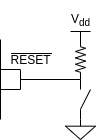
\includegraphics[width=75px]{images/16_Sleep_mode/reset_push_button.png}
    \end{figure}
    NB: a volte anche con un condensatore in parallelo al resistore.
    
    \item Watchdog Reset: è una periferica che periodicamente va contattata, se non lo si fa dopo un po' di tempo si ha un reset
    \item Brown-out Reset: quando la tensione scende un po' ma non va completamente a 0.
    In questi casi la CPU può commettere degli errori quindi un circuito analogico controlla la tensione e quando accade si ha un reset
    \item JTAG AVR Reset: reset inviato tramite una connessione JTAG
\end{itemize}

All' avvio del uC possiamo sapere quale sia stata la ragione del reset leggendo il registro MCUCSR:
\begin{figure}[H]
    \centering
    
\includegraphics[width=320px]{images/16_Sleep_mode/MCUCSR.png}
\end{figure}
\begin{itemize}
    \item JTRF: JTAG reset
    \item WDRF: watchdog reset
    \item BORF: Brown-out reset
    \item EXTRF: external reset
    \item PORF: power-on reset
\end{itemize}
